\section{Sensitivity} \label{sec:sensitivity}
Understanding the sensitivity of the GReX instrument to incoming signals is necessary for defining the strength of those signals and being able to place them in an astrophysical context.

The receiver gains and the system temperatures for the Cornell, OVRO, and Harvard stations are shown in \autoref{fig:Tsys}, computed using a Y-factor test (\autoref{eq:Trec}).
Sky measurements are taken before daybreak or after sundown to ensure emission from the sun does not enter the beam. 
This allows us to assume a constant sky temperature of $5.5\,\text{K}$, with $2.7\,\text{K}$ from the CMB, $1.9\,\text{K}$ from atmospheric effects, and $0.9\,\text{K}$ from galactic effects~\cite{levineGalacticNoisePassive2004}. 
We placed a slab of ambient-temperature (nominally $290\,\text{K}\pm5\,\text{K}$) radio-absorbent foam over the terminal antenna while taking hot data for the Y-factor test.
Data were saved in the Stokes I filterbank format for the hot foam and cold sky states.

\begin{figure}[h!]
    \centering
    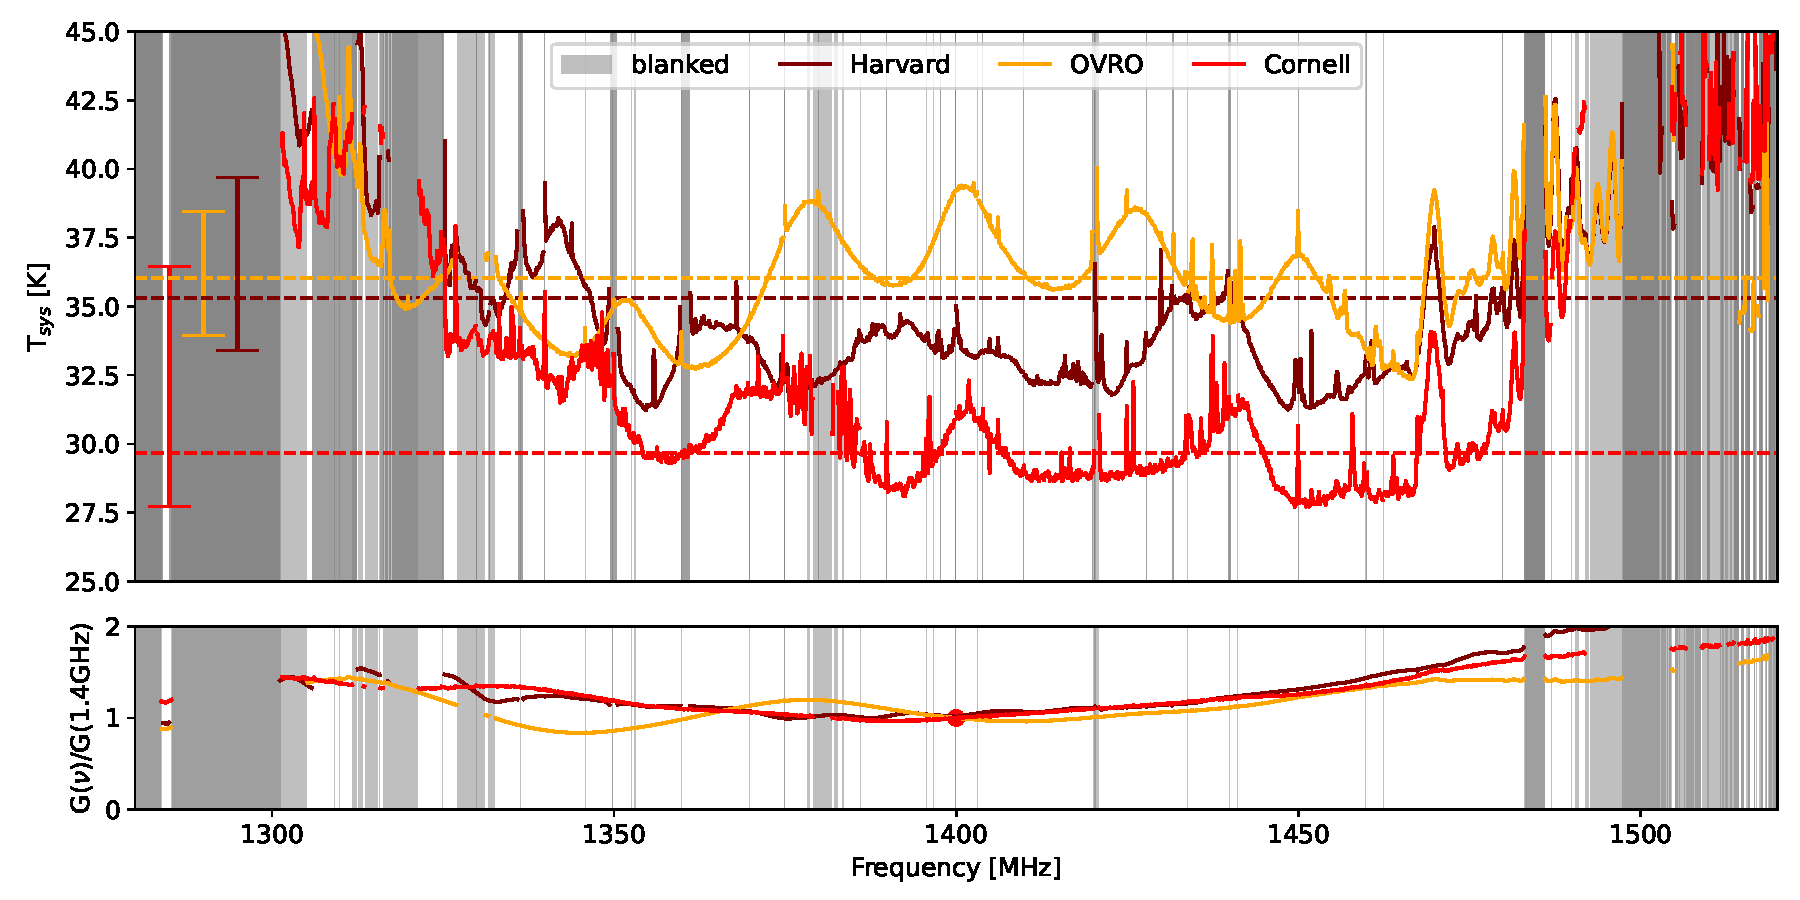
\includegraphics[width=\textwidth]{figures/Tsys.pdf}
    \caption[GReX system noise temperature]{System temperature and relative receiver gain measured for the GReX terminals at Cornell, OVRO, and Harvard.
    Dashed lines show the median system temperature with associated $16^{th}$ and $84^{th}$ quantile error bars.
    }
    \label{fig:Tsys}
\end{figure}

The system noise temperature for a GReX terminal is approximately $35\,\text{K}$, averaged across the band.
Obstructions in the beam such as buildings and trees will worsen the noise, as well as the presence of strong RFI desensitizing the receiver.
As such, optimal placement and configuration of attenuation/gains is critical to maximizing performance.
The second essential measure of system sensitivity is the forward gain ($g_f$) of the receiver. 
This quantity depends primarily on the integrated beam response function across the sky (\autoref{eq:FG}, \autoref{eq:Ae}), since that is the value mediating between the true brightness temperature integrated across the telescope beam and the nominal effective temperature representing the observed temperature (\autoref{eq:Teff}, \autoref{eq:Bnorm}).
Applying the effective area of the terminal found in \autoref{sec:beam_model} to \autoref{eq:FG}, we compute the forward gain as $g_f=84.2\,\text{kJy}\,\text{K}^{-1}\pm1.3\,\text{kJy}\,\text{K}^{-1}$.
Multiplying this value by the system temperature gives an SEFD of approximately $3\,\text{MJy}$.
When determining our detection threshold, we consider a proto-typical burst that fills the band and lasts $1\,\text{ms}$.
Our detectors are sensitive to an effective bandwidth of $188\,\text{MHz}$ ($75\%$ of the total bandwidth) and the use of matched-filtering with a set of boxcars in the detection pipeline allows our integration time to match the $1\,\text{ms}$ burst width. 
By averaging over these samples in frequency, time, and both polarizations, we find that for an event to attain an SNR of 10, it must have a corresponding flux density of at least $\sim50\,\text{kJy}$. 
This is a minimum requirement, as the angular deviation of a source away from the center of the detector beam at the time of observation increases the required flux density necessary to detect the burst.
